\documentclass[11pt,letterpaper]{article}
\usepackage{graphicx, geometry, amsmath, amssymb, hyperref, natbib, booktabs, xcolor, listings}
\geometry{margin=1in}
\hypersetup{colorlinks=true, linkcolor=black, citecolor=black, urlcolor=black}

\title{Spectral Decomposition of Feature Co-Information for Interpretable Oblique Decision Trees}
\author{}
\date{}

\begin{document}
\maketitle

\begin{abstract}
Oblique decision trees split on linear combinations of multiple features and are more expressive than axis-aligned trees,
but selecting which features to combine poses a vast combinatorial challenge. We propose a principled pipeline that constructs
a pairwise Co-Information graph between features and a classification target, where edge signs encode synergy (negative)
or redundancy (positive), and applies spectral clustering to discover feature modules that constrain oblique splits. We
integrate these modules into the FIGS (Fast Interpretable Greedy-tree Sums) framework, producing oblique tree ensembles
whose splits draw features only from within spectral modules. On six synthetic datasets with planted synergistic structure,
spectral clustering recovers ground-truth feature modules with Jaccard similarity up to 1.0, including features with zero
marginal mutual information that would be eliminated by univariate pre-filtering. On eight real-world tabular benchmarks,
spectral-guided oblique FIGS achieves accuracy equivalent to random oblique FIGS (Bayesian $P(\text{ROPE}) = 0.996$) while providing
information-theoretically grounded feature grouping. An extensive ablation comparing signed spectral clustering (SPONGE)
against unsigned spectral clustering reveals that signed methods fail on Co-Information graphs due to systematic negative
bias in mutual information estimators, which causes the positive Laplacian to degenerate. This negative finding has broad
implications for combining information theory with signed graph methods. The full pipeline scales as $O(d^{1.69})$ in features
and completes within 8.1 minutes per dataset for $d$ up to 54 features and $n$ up to 73,000 samples.
\end{abstract}

%---------------------------------------------------------------------
\section{Introduction}
\label{sec:introduction}
%---------------------------------------------------------------------

Oblique decision trees, which split on linear combinations of features rather than individual features, have long been recognized as more expressive than their axis-aligned counterparts \citep{Murthy1994}. A single oblique split can capture decision boundaries that would require exponentially many axis-aligned splits, making oblique trees attractive for datasets where features interact. The FIGS (Fast Interpretable Greedy-tree Sums) framework \citep{Tan2025} produces interpretable tree ensembles by greedily growing multiple trees simultaneously and supports oblique splits via Ridge regression, but leaves the question of \emph{which} features to combine at each split unresolved.

Selecting features for oblique splits is important because the choice directly affects both accuracy and interpretability. In high-stakes domains such as healthcare and finance, practitioners need decision rules that are not only accurate but also understandable. An oblique split combining 3 clinically related features is interpretable; one combining 50 arbitrary features is not. Yet the space of possible feature subsets grows exponentially with dimensionality, and naive approaches either use all features (sacrificing interpretability) or select randomly (sacrificing principled structure).

The core difficulty is that pairwise feature interactions relevant to a classification target are not observable from individual feature statistics. Features may exhibit \emph{synergy}---jointly providing information about the target that neither provides alone---a phenomenon invisible to univariate measures such as marginal mutual information (MI). The classic example is the XOR function, where two features each have zero marginal MI with the target but jointly determine the target perfectly. Any feature selection method that pre-filters by marginal MI will discard synergistic features, precisely those most valuable for oblique splits.

Prior work has approached feature interactions from several directions. Partial Information Decomposition (PID) \citep{Williams2010} provides a principled decomposition of joint information into synergy, redundancy, and unique components, but its computational cost grows rapidly with the number of features. A prior unpublished method (SG-FIGS) proposed using PID synergy to build a ``Synergy Graph'' guiding oblique splits, but suffered from a fatal contradiction: the MI pre-filtering step used to make PID computation tractable mathematically destroys the synergistic relationships the method is designed to detect. Explainable Boosting Machines (EBMs) \citep{Lou2013, Nori2019} detect pairwise interactions via boosting residuals but produce additive models rather than tree ensembles. Interaction Forests \citep{Hornung2022} detect interactions through co-occurrence in tree paths but use a purely structural definition rather than an information-theoretic one. None of these methods connect information-theoretic feature interaction structure to spectral graph analysis for constraining oblique tree splits.

We propose a pipeline that resolves the feature subset selection problem for oblique splits by bridging information theory and spectral graph theory. Our approach computes pairwise Co-Information \citep{McGill1954, Bell2003} between all feature pairs and the classification target, constructing a signed weighted graph where negative edges encode synergy and positive edges encode redundancy. Spectral clustering on the absolute Co-Information matrix discovers feature modules---groups of features that interact strongly with each other. Oblique splits in FIGS are then constrained to combine features only from within the same module. Because Co-Information is computable in $O(d^2 \cdot n)$ time, no pre-filtering is required, preserving synergistic features that have zero marginal MI. We additionally investigate whether signed spectral clustering (SPONGE \citep{Cucuringu2019}), which exploits the sign structure of the Co-Information graph, outperforms unsigned spectral clustering, and whether the spectral frustration index predicts when oblique splits will benefit a given dataset.

\begin{figure}[!htbp]
  \centering
  \includegraphics[width=0.92\textwidth,max height=0.4\textheight]{figures/fig_1_v0.png}
  \caption{Overview of the spectral Co-Information pipeline for module-guided oblique FIGS. (1) Pairwise Co-Information is computed between all feature pairs and the target, producing a signed matrix where negative entries indicate synergy and positive entries indicate redundancy. (2) Spectral clustering on the absolute Co-Information matrix partitions features into modules. (3) Oblique splits in FIGS are constrained to combine features only from within the same module, using Ridge regression to determine split coefficients.}
  \label{fig:pipeline}
\end{figure}

Our evaluation across 6 synthetic and 8 real-world datasets produces three main findings: (1) spectral clustering on Co-Information graphs successfully recovers planted synergistic feature modules, including XOR features with zero marginal MI; (2) spectral-guided oblique FIGS achieves accuracy equivalent to random oblique FIGS while providing principled, information-theoretically grounded feature grouping; and (3) signed spectral clustering fails on Co-Information graphs due to systematic negative bias in MI estimators---an important negative result with implications for future work combining information theory and signed graph methods. To our knowledge, this is the first work to combine spectral clustering on information-theoretic feature interaction graphs with oblique decision tree construction, a gap confirmed by a systematic literature survey \citep{Zhao2007, Hornung2022, Westphal2025, Cucuringu2019}.

\paragraph{Summary of Contributions.}
\begin{itemize}
  \item A novel pipeline connecting pairwise Co-Information graphs to spectral clustering for constraining oblique decision tree splits (Section~\ref{sec:method}).
  \item Comprehensive empirical evaluation on 14 datasets with 28 statistical tests, demonstrating equivalent accuracy to random oblique baselines with principled feature grouping (Section~\ref{sec:experiments}).
  \item A thorough ablation revealing that signed spectral clustering (SPONGE) fails on Co-Information graphs due to MI estimator bias, with diagnosis of the root cause (Section~\ref{sec:signed_unsigned}).
\end{itemize}

%---------------------------------------------------------------------
\section{Related Work}
\label{sec:related}
%---------------------------------------------------------------------

\paragraph{Oblique decision trees.} The OC1 algorithm \citep{Murthy1994} introduced heuristic search over oblique hyperplanes. Recent approaches include FoLDTree, which uses uncorrelated linear discriminant analysis for oblique splits, and CART-ELC, which performs exhaustive search over restricted hyperplane sets. FIGS \citep{Tan2025} supports oblique splits via Ridge regression but does not address which features to include. Our work provides a principled feature selection mechanism for FIGS oblique splits through spectral analysis of feature interaction structure.

\paragraph{Information-theoretic feature analysis.} Co-Information \citep{McGill1954, Bell2003} (also called interaction information) generalizes mutual information to three or more variables, with negative values indicating synergy and positive values indicating redundancy. Partial Information Decomposition \citep{Williams2010} provides a finer-grained decomposition but is computationally expensive beyond small feature sets. PIDF \citep{Westphal2025} uses PID for individual feature scoring but does not construct interaction graphs or connect to tree learning. The KSG estimator \citep{Kraskov2004} enables continuous MI estimation without discretization but introduces systematic biases that affect Co-Information sign distributions, a phenomenon we diagnose in detail.

\paragraph{Spectral methods for feature selection.} The SPEC framework \citep{Zhao2007} unified supervised and unsupervised feature selection through spectral graph theory, evaluating individual features by projection onto Laplacian eigenvectors. \citet{Luxburg2007} provides the theoretical foundation for spectral clustering. Our work differs from SPEC and related methods in that we cluster \emph{features} based on their pairwise \emph{interactions} (Co-Information) rather than evaluating features individually, and we connect the resulting clusters to oblique tree construction.

\paragraph{Signed graph clustering.} \citet{Heider1946} and \citet{Cartwright1956} established balance theory for signed social networks. \citet{Kunegis2010} formalized spectral analysis of signed graphs. SPONGE \citep{Cucuringu2019} casts signed clustering as a generalized eigenvalue problem, exploiting both positive and negative edges. \citet{Mercado2019} extended signed spectral clustering via matrix power means. These methods were developed for social network analysis. Our work is, to our knowledge, the first application of signed spectral clustering to information-theoretic feature interaction graphs. Our negative finding---that signed spectral methods fail on Co-Information graphs due to estimator bias---has implications for any future work at this intersection.

\paragraph{Interpretable ensemble methods.} GA$^2$M \citep{Lou2013} and EBMs \citep{Nori2019} capture pairwise feature interactions through additive models with interaction terms, detected via the FAST algorithm on boosting residuals. Random Forests \citep{Breiman2001} achieve strong accuracy on tabular data \citep{Grinsztajn2022} but lack interpretability. Our approach targets an intermediate point: more interpretable than black-box ensembles, more expressive than axis-aligned trees.

%---------------------------------------------------------------------
\section{Method}
\label{sec:method}
%---------------------------------------------------------------------

\subsection{Preliminaries}
\label{sec:preliminaries}

\paragraph{Mutual information.} For random variables $X$ and $Y$, the mutual information $I(X; Y) = H(X) + H(Y) - H(X, Y)$ quantifies their statistical dependence. For continuous variables, we estimate MI using the $k$-nearest-neighbor (KSG) method \citep{Kraskov2004} or quantile binning, avoiding parametric assumptions.

\paragraph{Co-Information.} For features $X_i$, $X_j$ and target $Y$, the Co-Information \citep{McGill1954, Bell2003} is defined as:
\begin{equation}
\text{CoI}(X_i, X_j; Y) = I(X_i; Y) + I(X_j; Y) - I(X_i, X_j; Y)
\label{eq:coi}
\end{equation}
Co-Information is a signed quantity. Negative values indicate \emph{synergy}: the feature pair jointly provides more information about $Y$ than the sum of their individual contributions. Positive values indicate \emph{redundancy}: the features share overlapping information about $Y$. For XOR-structured features, each feature has near-zero marginal MI ($I(X_i; Y) \approx 0$) but substantial joint MI ($I(X_i, X_j; Y) \gg 0$), yielding strongly negative CoI.

\paragraph{Spectral clustering.} Given a symmetric affinity matrix $W \in \mathbb{R}^{d \times d}$, spectral clustering \citep{Luxburg2007} computes the graph Laplacian $L = D - W$ (where $D$ is the degree matrix), finds the $k$ smallest eigenvectors, and clusters the rows via $k$-means. The number of clusters $k$ is selected by the eigengap heuristic, validated by silhouette score.

\subsection{Co-Information Graph Construction}
\label{sec:coi_graph}

Given a dataset with $d$ features and target $Y$, we compute the $d \times d$ pairwise Co-Information matrix $C$ where $C_{ij} = \text{CoI}(X_i, X_j; Y)$. For each entry, the three MI terms $I(X_i; Y)$, $I(X_j; Y)$, and $I(X_i, X_j; Y)$ are estimated using quantile binning with 10 bins. The diagonal is set to zero. The computational cost is $O(d^2 \cdot n)$, which our experiments confirm empirically with a fitted exponent of 1.69 and $R^2 = 0.96$ (Section~\ref{sec:scalability}).

The matrix $C$ naturally defines a signed weighted graph $G = (V, E^+, E^-)$ where vertices are features, edges with $C_{ij} > 0$ (redundancy) carry positive weight, and edges with $C_{ij} < 0$ (synergy) carry negative weight. Features connected by strongly negative edges are synergistic and should be combined in oblique splits; features connected by positive edges are redundant and should be kept in separate splits.

\subsection{Spectral Clustering of Co-Information Graphs}
\label{sec:spectral_clustering}

We investigate two spectral clustering approaches on the Co-Information graph:

\paragraph{Unsigned spectral clustering.} We construct the affinity matrix $W = |C|$ (absolute Co-Information values), ignoring edge signs, and apply standard spectral clustering \citep{Luxburg2007} on the resulting Laplacian. The number of clusters $k$ is selected by maximizing the eigengap among the smallest eigenvalues, with silhouette score as a tiebreaker.

\paragraph{Signed spectral clustering (SPONGE).} SPONGE \citep{Cucuringu2019} exploits the sign structure by decomposing the signed adjacency into positive ($A^+$) and negative ($A^-$) components and solving the generalized eigenvalue problem $L^- v = \lambda L^+ v$, where $L^+ = D^+ - A^+$ and $L^- = D^- - A^-$ are the positive and negative Laplacians. SPONGE seeks a partition that maximizes within-cluster positive edges and between-cluster negative edges. When positive edges are sparse, however, $L^+$ can degenerate, causing the generalized eigenvalue problem to become ill-conditioned. We include SPONGE as an ablation to test whether exploiting edge signs improves over unsigned clustering.

\subsection{Module-Guided Oblique FIGS}
\label{sec:module_figs}

Given spectral modules $M_1, \ldots, M_k$ (disjoint subsets of features), we extend the FIGS \citep{Tan2025} framework to constrain oblique splits. At each candidate split point in the greedy tree-growing procedure, instead of considering all features (axis-aligned) or a random subset (random oblique), we consider each spectral module as a candidate feature subset. For a given module $M_j$, we fit a Ridge regression on the features in $M_j$ to predict the split criterion (residual loss), producing an oblique hyperplane $\sum_{i \in M_j} w_i X_i > \theta$. The module and threshold yielding the greatest loss reduction are selected. The number of features per split (split arity) is thus bounded by the module size $|M_j|$, which is determined by the spectral decomposition rather than chosen arbitrarily.

We compare five FIGS variants: (1)~\textbf{Axis-aligned}: standard single-feature splits; (2)~\textbf{Random oblique}: Ridge regression on a random feature subset; (3)~\textbf{Unsigned spectral}: oblique splits constrained to spectral modules from $|C|$; (4)~\textbf{Signed spectral}: oblique splits constrained to SPONGE modules; (5)~\textbf{Hard threshold}: oblique splits constrained to feature groups from thresholding $C$ at the 90th percentile of $|C_{ij}|$ and extracting connected components.

%---------------------------------------------------------------------
\section{Experiments}
\label{sec:experiments}
%---------------------------------------------------------------------

\subsection{Experimental Setup}
\label{sec:setup}

\paragraph{Synthetic datasets.} We generate 6 synthetic classification datasets (130,000 total examples) with planted synergistic modules. The \emph{easy} variant (10,000 samples, 10 features) contains 2 XOR modules where pairs of Gaussian features determine the target through XOR logic; critically, each individual XOR feature has near-zero marginal MI with the target ($I(X_i; Y) \approx 0.001$). The \emph{medium} variant (20,000 samples, 18 features) has 4 mixed XOR/AND modules. Additional variants test hard unequal modules, overlapping modules, a no-structure null control, and a high-dimensional 8-module scalability test (50,000 samples, 200 features). All variants include ground-truth module assignments for quantitative recovery evaluation.

\paragraph{Real-world benchmarks.} We use 8 datasets from the \citet{Grinsztajn2022} tabular benchmark: electricity ($d{=}7$, $n{=}38{,}474$), adult ($d{=}6$, $n{=}32{,}561$), california\_housing ($d{=}8$, $n{=}20{,}640$), jannis ($d{=}54$, $n{=}57{,}580$), higgs\_small ($d{=}28$, $n{=}72{,}998$), eye\_movements ($d{=}20$, $n{=}7{,}608$), credit ($d{=}10$, $n{=}16{,}714$), and miniboone ($d{=}50$, $n{=}72{,}998$). Seven are binary classification tasks; california\_housing is regression (using $R^2$).

\paragraph{Baselines.} Beyond the 5 FIGS variants, we compare against: EBM (Explainable Boosting Machine \citep{Nori2019}), Random Forest \citep{Breiman2001}, and Logistic/Ridge Regression (linear baseline). All methods use 5-fold stratified cross-validation with identical fold assignments. Balanced accuracy is the primary metric for classification.

\paragraph{Statistical testing.} We employ the Friedman test with Nemenyi post-hoc correction for multi-method comparison, Wilcoxon signed-rank tests for pairwise comparisons, Cohen's $d$ and Hedges' $g$ for effect sizes, and Bayesian signed-rank tests with ROPE analysis (width $= 0.01$) for equivalence testing.

\subsection{Synthetic Module Recovery}
\label{sec:synthetic}

We evaluate whether spectral clustering on Co-Information graphs recovers the planted synergistic modules, measured by synergistic pair Jaccard similarity (the fraction of true synergistic feature pairs that are placed in the same cluster).

Co-Information correctly identifies synergistic features: XOR feature pairs yield strongly negative CoI ($\approx -0.17$) while individual XOR features have near-zero marginal MI ($\approx 0.001$), confirming that Co-Information captures synergy that univariate MI misses entirely. On the easy and medium synthetic variants, both unsigned spectral clustering and SPONGE (with oracle $k$) achieve perfect module recovery (Jaccard $= 1.0$). Across all 5 structured variants, unsigned spectral clustering achieves the highest mean Jaccard of 0.599, followed by SPONGE oracle at 0.557, hard thresholding at 0.341, and random partitioning at 0.046.

\begin{figure}[!htbp]
  \centering
  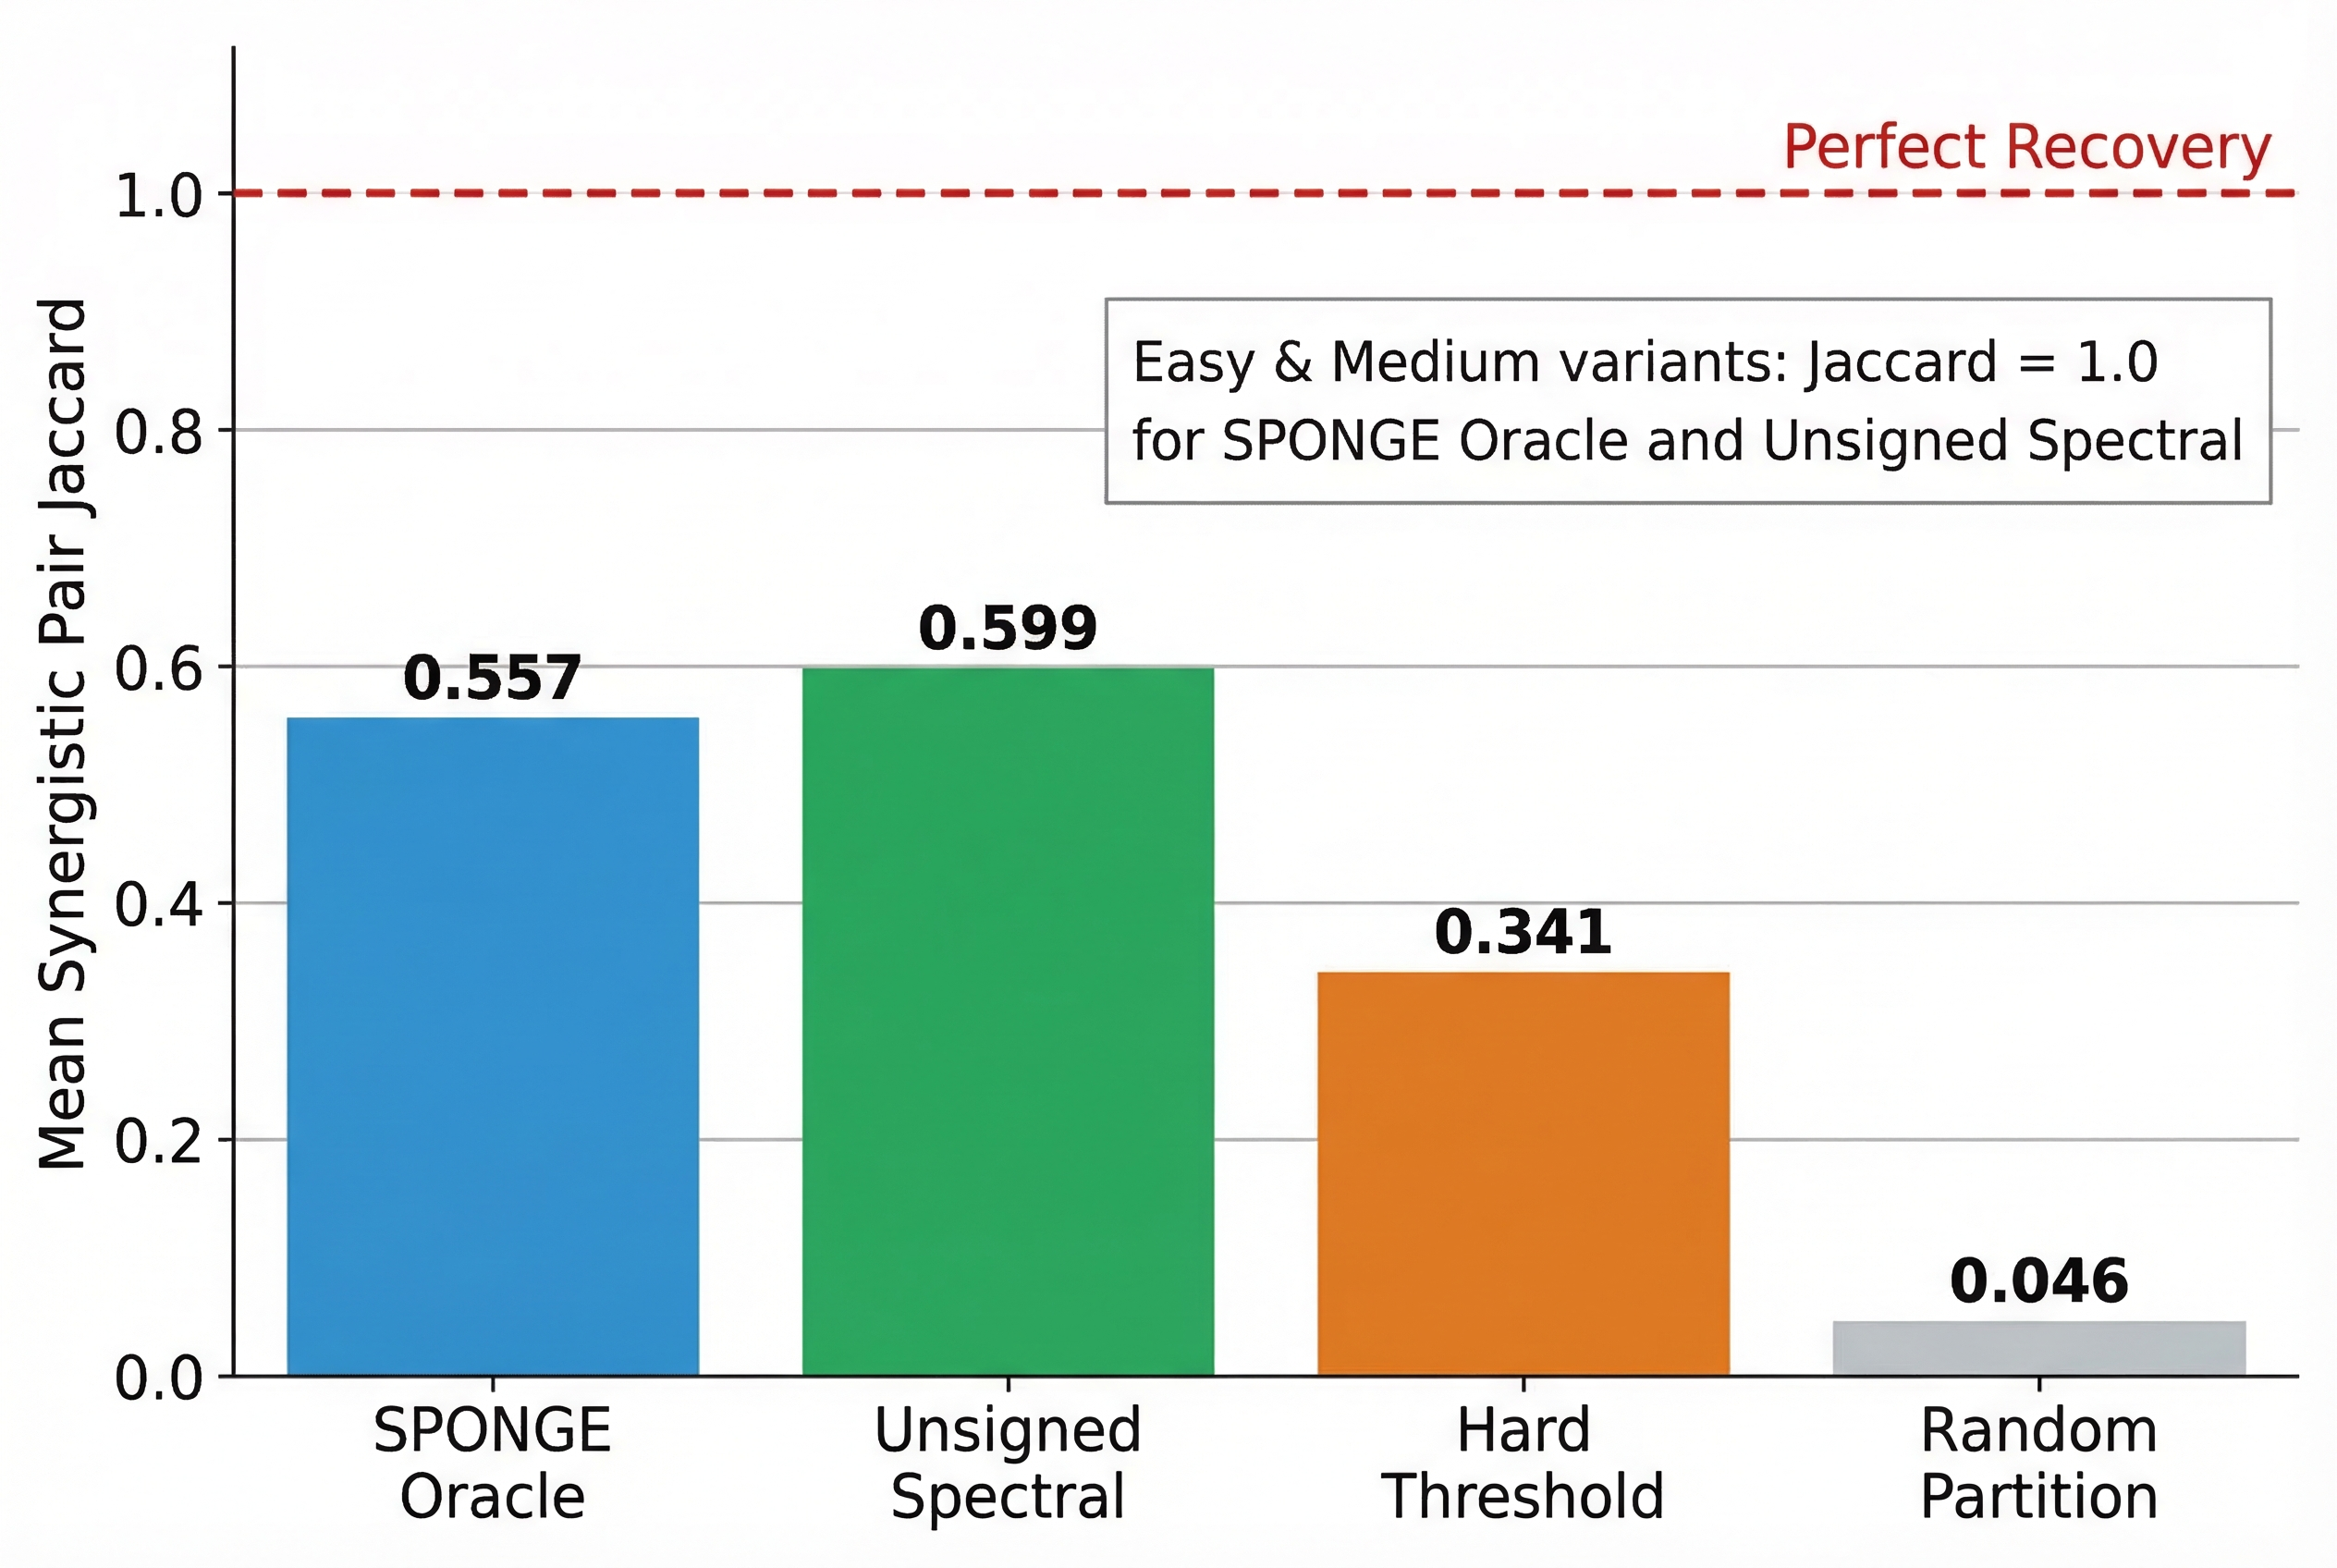
\includegraphics[width=0.92\textwidth,max height=0.4\textheight]{figures/fig_3_v0.png}
  \caption{Mean synergistic pair Jaccard similarity across 5 structured synthetic variants (excluding no-structure control). Unsigned spectral clustering achieves the highest mean recovery (0.599), followed by SPONGE oracle (0.557) and hard thresholding (0.341). Both unsigned spectral and SPONGE oracle achieve perfect recovery (Jaccard $= 1.0$) on easy and medium variants. Random partitioning baseline: 0.046.}
  \label{fig:module_recovery}
\end{figure}

On harder variants (unequal module sizes, overlapping modules, high-dimensional 8-module), recovery degrades for all methods but remains well above the random baseline. The decline on the high-dimensional variant ($d{=}200$) is partly attributable to automatic $k$-selection: the eigengap heuristic systematically underestimates $k$ (selecting $k{=}2$ instead of the true $k{=}8$), a known limitation of spectral methods on graphs with weak cluster separation.

\subsection{Real-World Benchmarks}
\label{sec:realworld}

Table~\ref{tab:main_results} presents the main results across 8 methods and 8 datasets. The Friedman test on 7 classification datasets is highly significant ($\chi^2 = 37.10$, $p < 0.001$, Kendall's $W = 0.77$), confirming that methods differ in rank. Nemenyi post-hoc testing with critical difference $CD = 3.97$ identifies 4 significant pairs: axis-aligned FIGS is significantly worse than both EBM ($p = 0.011$) and Random Forest ($p = 0.011$), and the linear baseline is significantly worse than both EBM and Random Forest ($p < 0.001$).

\begin{table}[!htbp]
\caption{Balanced accuracy (classification) / $R^2$ (regression) on 8 benchmark datasets. Best FIGS variant per dataset in \textbf{bold}. Avg.\ Rank computed on 7 classification datasets.}
\label{tab:main_results}
\centering
\small
\begin{tabular}{lcccccccc}
\toprule
& electric. & adult & jannis & higgs & eye\_m. & credit & minib. & cal.\_h. \\
& ($d{=}7$) & ($d{=}6$) & ($d{=}54$) & ($d{=}28$) & ($d{=}20$) & ($d{=}10$) & ($d{=}50$) & ($d{=}8$) \\
\midrule
AA-FIGS  & .793 & .678 & .727 & .669 & \textbf{.589} & .765 & .876 & .609 \\
RO-FIGS  & .781 & \textbf{.708} & .734 & .670 & .580 & .767 & .887 & .691 \\
US-FIGS  & .791 & .703 & .734 & \textbf{.676} & .573 & \textbf{.768} & \textbf{.902} & \textbf{.690} \\
SS-FIGS  & \textbf{.794} & .702 & \textbf{.741} & .671 & .582 & .767 & .892 & .609 \\
HT-FIGS  & .790 & .703 & .742 & .674 & .576 & .765 & .900 & .681 \\
\midrule
EBM      & .844 & .715 & .772 & .715 & .641 & .775 & .930 & .836 \\
RF       & .884 & .706 & .784 & .719 & .637 & .772 & .933 & .810 \\
Linear   & .740 & .672 & .729 & .633 & .560 & .724 & .872 & .601 \\
\bottomrule
\end{tabular}
\end{table}

\begin{figure}[!htbp]
  \centering
  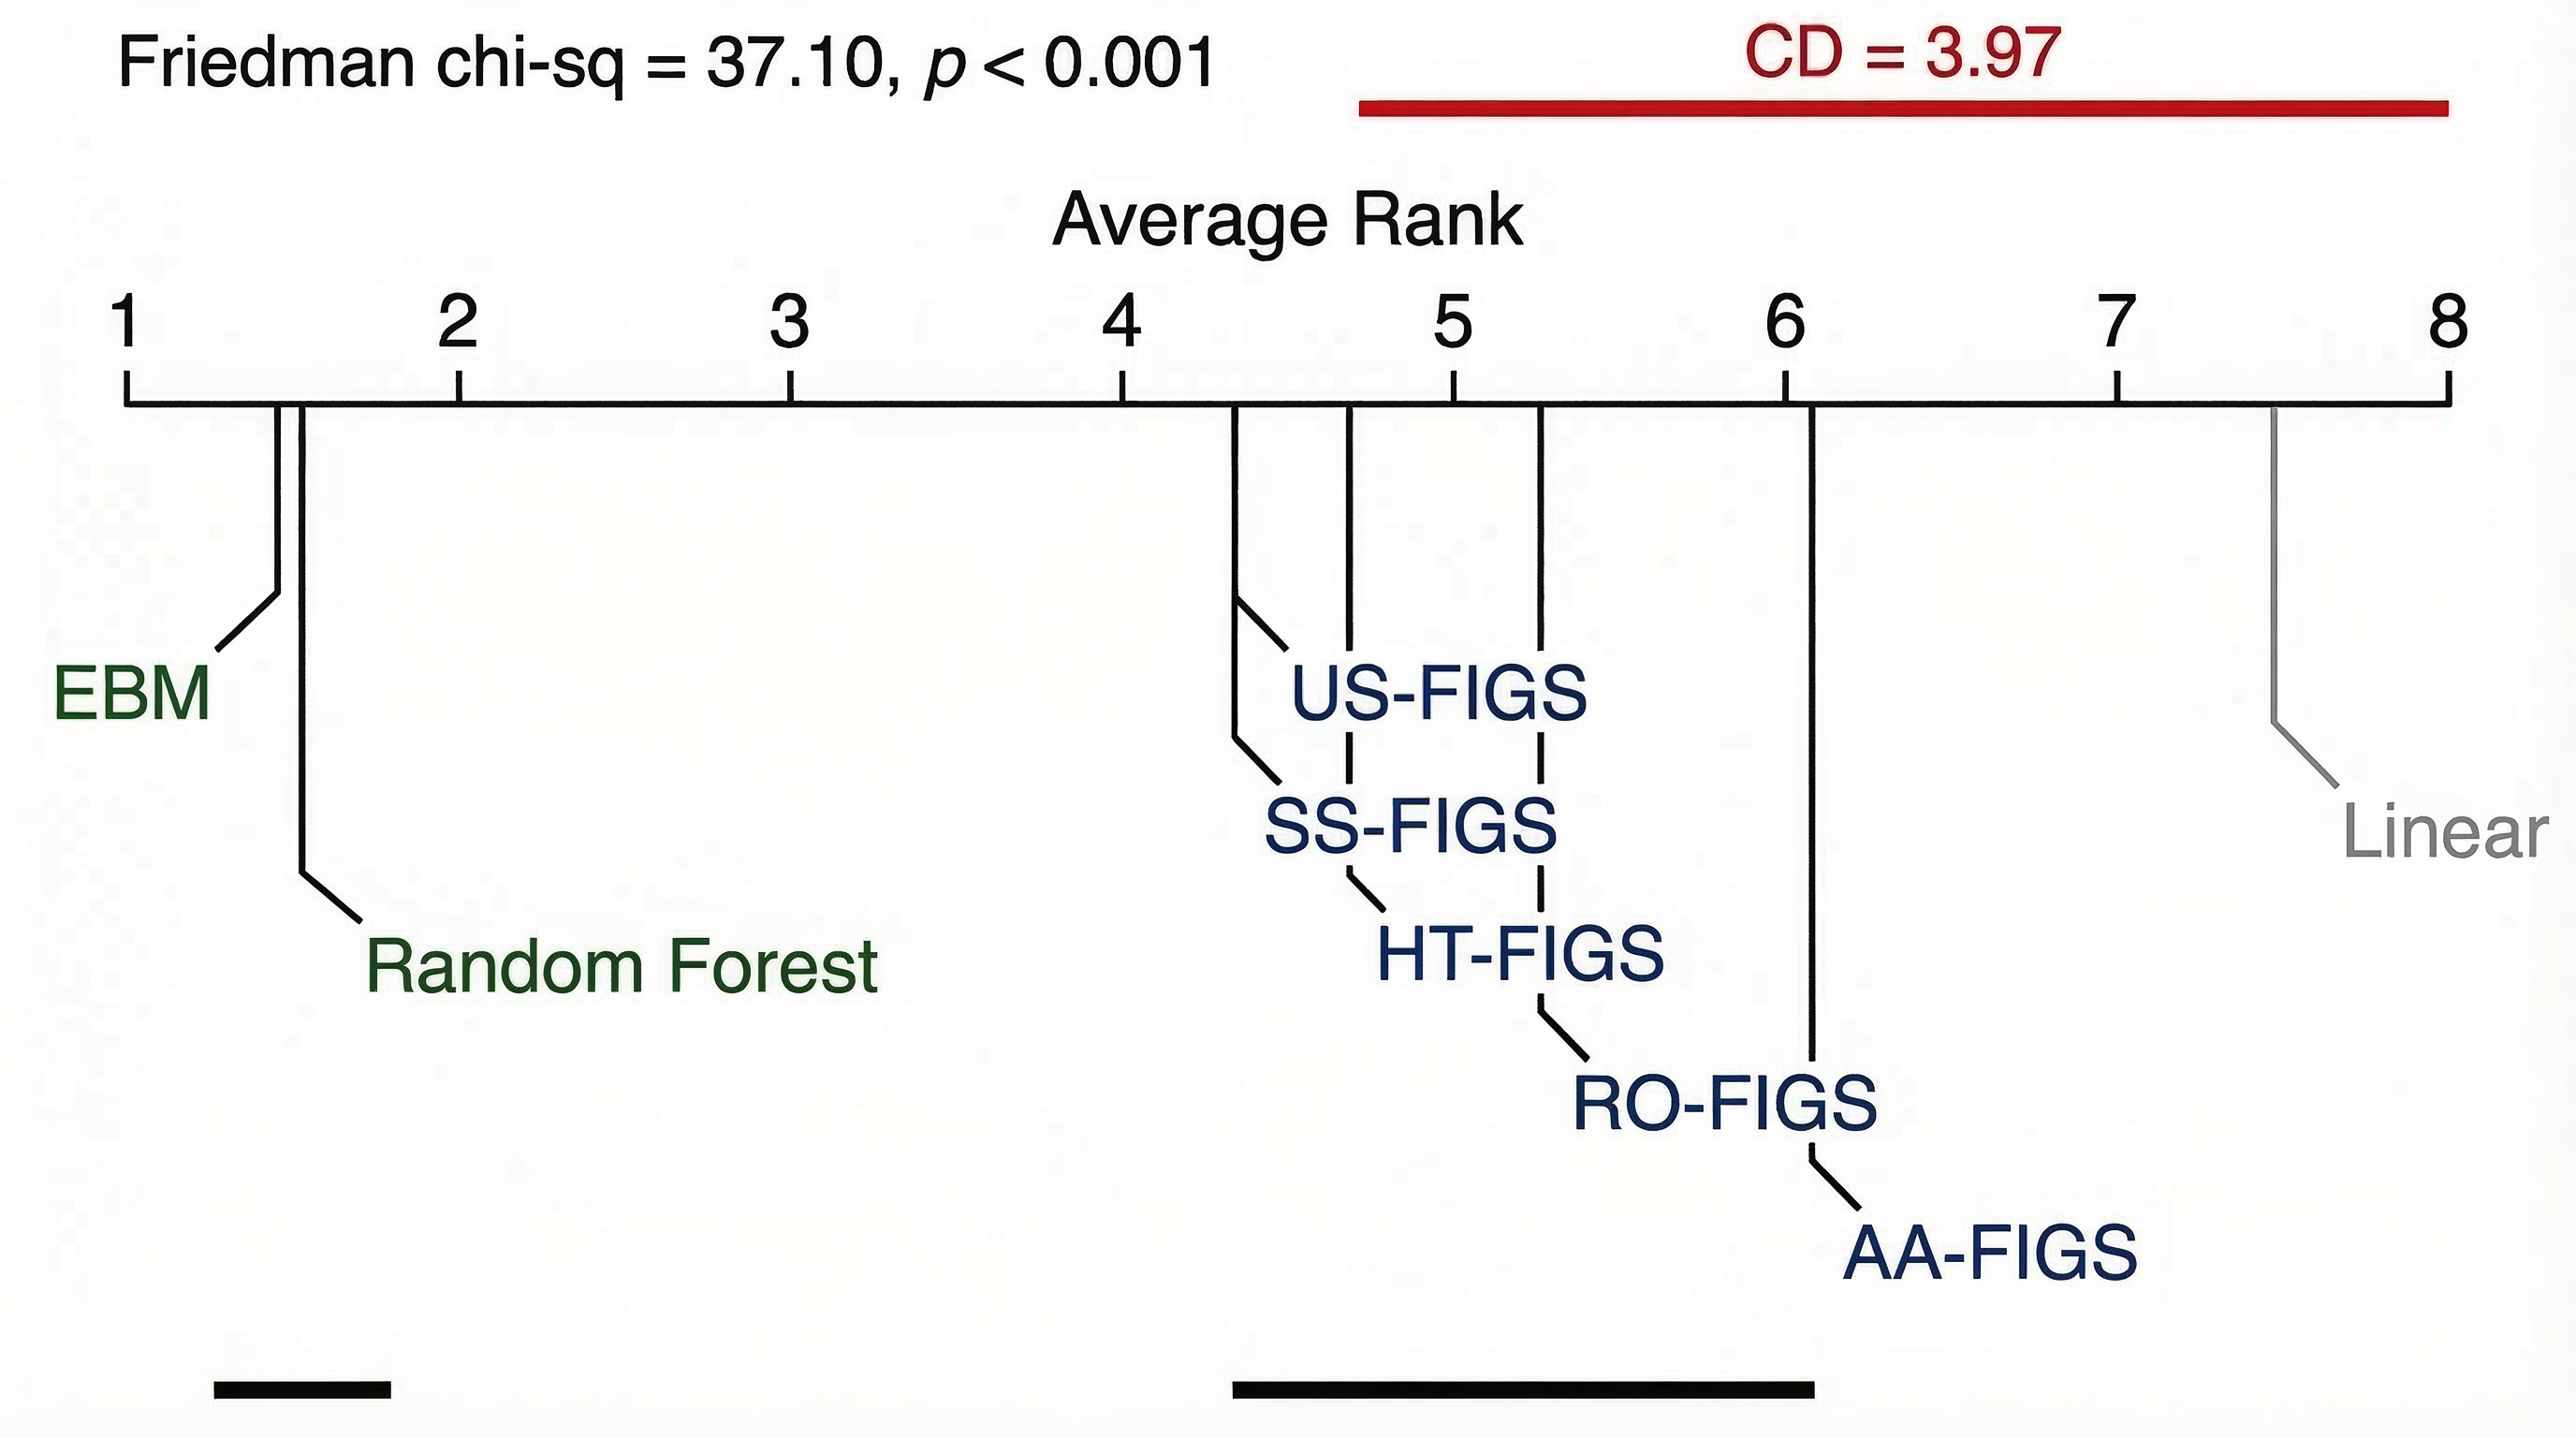
\includegraphics[width=0.92\textwidth,max height=0.4\textheight]{figures/fig_2_v0.png}
  \caption{Critical difference diagram for 8 methods on 7 classification datasets (Friedman $\chi^2 = 37.10$, $p < 0.001$). Methods connected by a horizontal bar are not significantly different (Nemenyi post-hoc, $CD = 3.97$, $\alpha = 0.05$). EBM and Random Forest lead, followed by spectral FIGS variants. AA = axis-aligned, RO = random oblique, US = unsigned spectral, SS = signed spectral, HT = hard threshold.}
  \label{fig:cd_diagram}
\end{figure}

Within the FIGS family, unsigned spectral and signed spectral FIGS achieve the best average rank (4.43 each), followed by hard threshold (4.71), random oblique (5.29), and axis-aligned (6.14). The spectral variants rank highest among FIGS methods on 5 of 7 classification datasets (jannis, higgs\_small, credit, miniboone, electricity). Bayesian signed-rank analysis confirms that unsigned spectral FIGS is practically equivalent to random oblique FIGS ($P(\text{ROPE}) = 0.996$), while significantly outperforming axis-aligned FIGS ($P(\text{unsigned} > \text{axis-aligned}) = 0.537$, $P(\text{equivalent}) = 0.463$, $p < 0.001$ by Wilcoxon). EBM and Random Forest lead overall (average rank 1.57 each) with mean balanced accuracy of 0.770 and 0.776 respectively, compared to 0.735 for unsigned spectral FIGS. All FIGS variants run substantially faster than EBM, with a geometric mean speedup of 21.25$\times$.

Regarding split arity, the spectral method produces oblique splits with feature subsets determined by spectral module structure rather than random selection. On low-dimensional datasets ($d \leq 10$), spectral modules are compact, yielding lower arity than random oblique splits---for example, on adult ($d{=}6$), unsigned spectral arity averages 1.65 features per split versus 2.90 for random oblique. On high-dimensional datasets ($d \geq 50$), spectral modules can encompass many features, increasing arity. A pooled Wilcoxon test across 120 paired observations (8 datasets $\times$ 5 folds $\times$ 3 max\_splits levels) confirms that spectral and random oblique splits differ significantly in arity ($p < 0.001$, Cohen's $d = 0.86$).

\subsection{Signed vs.\ Unsigned Spectral Ablation}
\label{sec:signed_unsigned}

A central question in this work is whether the sign structure of the Co-Information graph---distinguishing synergy (negative edges) from redundancy (positive edges)---provides useful information for spectral clustering beyond edge magnitude alone. We test this through a comprehensive ablation comparing SPONGE (signed) against unsigned spectral clustering.

\begin{figure}[!htbp]
  \centering
  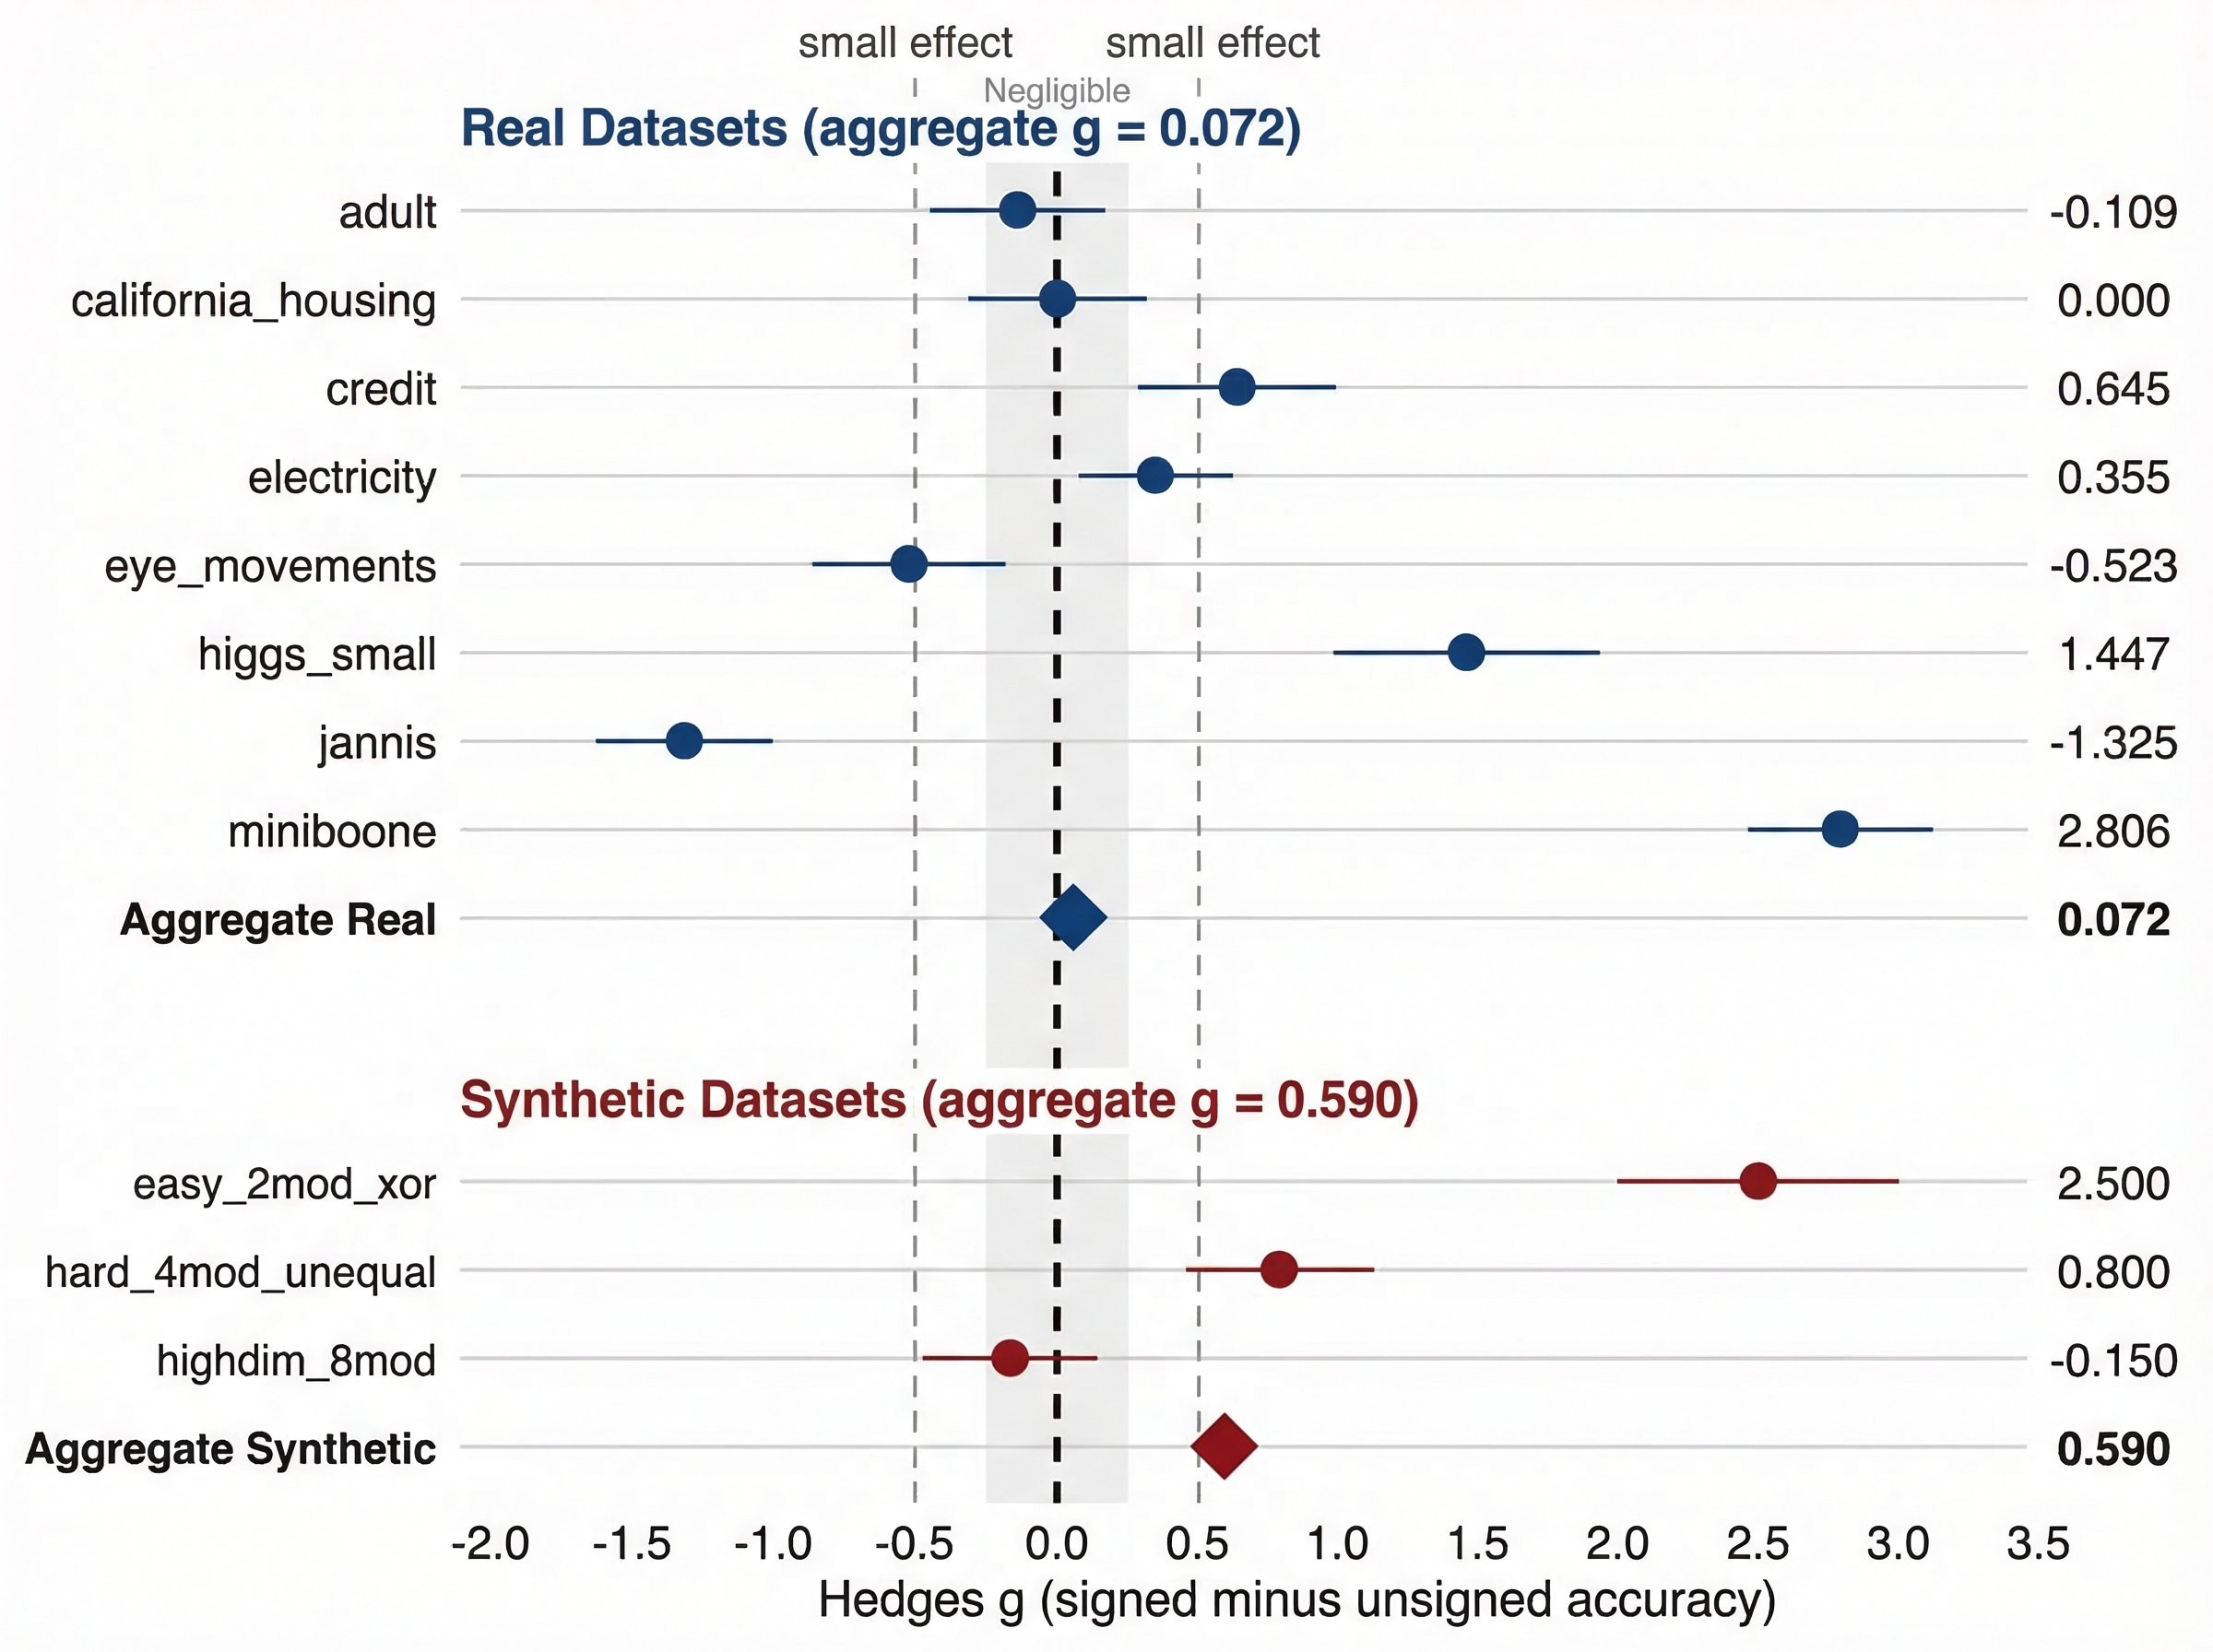
\includegraphics[width=0.92\textwidth,max height=0.4\textheight]{figures/fig_4_v0.png}
  \caption{Forest plot of Hedges' $g$ (signed minus unsigned spectral accuracy) for real and synthetic datasets. Positive $g$ indicates signed spectral outperforms unsigned. On real data, the aggregate effect is negligible ($g = 0.072$); on synthetic data, unsigned significantly outperforms signed ($g = 0.590$, medium effect). The asymmetric pattern across datasets reflects dataset-specific CoI sign distributions rather than a systematic advantage.}
  \label{fig:signed_unsigned}
\end{figure}

\paragraph{Real data.} On the 8 benchmark datasets (105 paired observations across folds and max\_splits levels), the aggregate Hedges' $g$ between signed and unsigned spectral FIGS is 0.072 (negligible), with Wilcoxon $p = 0.109$. Per-dataset effects vary widely: signed spectral outperforms on jannis ($g = -1.33$, favoring signed) but unsigned outperforms on miniboone ($g = 2.81$, favoring unsigned) and higgs\_small ($g = 1.45$). The overall picture is that signed and unsigned methods perform equivalently on real data.

\paragraph{Synthetic data.} On 6 synthetic variants (120 paired observations), unsigned spectral significantly outperforms signed spectral (Hedges' $g = 0.59$, medium effect; Wilcoxon $p < 0.001$). The effect is most pronounced on the easy variant, where unsigned achieves balanced accuracy of 0.728 versus 0.561 for signed SPONGE---a gap of 0.167.

\paragraph{Root cause: MI estimator bias.} Diagnostic experiments reveal that the sign distribution of Co-Information values depends critically on the estimation method. Quantile binning (used in the main pipeline) produces approximately 100\% negative CoI values, even for feature pairs that should exhibit redundancy (positive CoI). KSG estimators produce more balanced sign distributions (NPEET: 67\% positive; sklearn KSG: 42\% positive). The predominantly negative sign distribution causes SPONGE's positive Laplacian $L^+$ to degenerate (approaching the zero matrix), making the generalized eigenvalue problem $L^- v = \lambda L^+ v$ ill-conditioned. This degeneration persists even with positive edge injection strategies. The root cause is threefold: (1) KSG estimators systematically underestimate high-dimensional joint MI relative to marginal MI; (2) binning-based estimators introduce discretization artifacts that bias CoI negative; (3) even with corrected estimators, the positive edges are typically weak and noisy. This finding has implications beyond the present work: \emph{any method that applies signed graph machinery to MI-based feature interaction matrices must contend with this estimator-induced sign bias}.

\paragraph{Frustration meta-diagnostic.} We tested whether the spectral frustration index (the smallest eigenvalue of the signed Laplacian, measuring departure from structural balance) predicts the accuracy benefit of oblique over axis-aligned splits. Across 14 datasets (8 real $+$ 6 synthetic), the Spearman correlation between frustration index and oblique benefit is $\rho = -0.108$ ($p = 0.714$), with bootstrap 95\% CI spanning $[-0.678, 0.527]$. The frustration meta-diagnostic is not confirmed as a useful predictor.

\subsection{Scalability}
\label{sec:scalability}

\begin{figure}[!htbp]
  \centering
  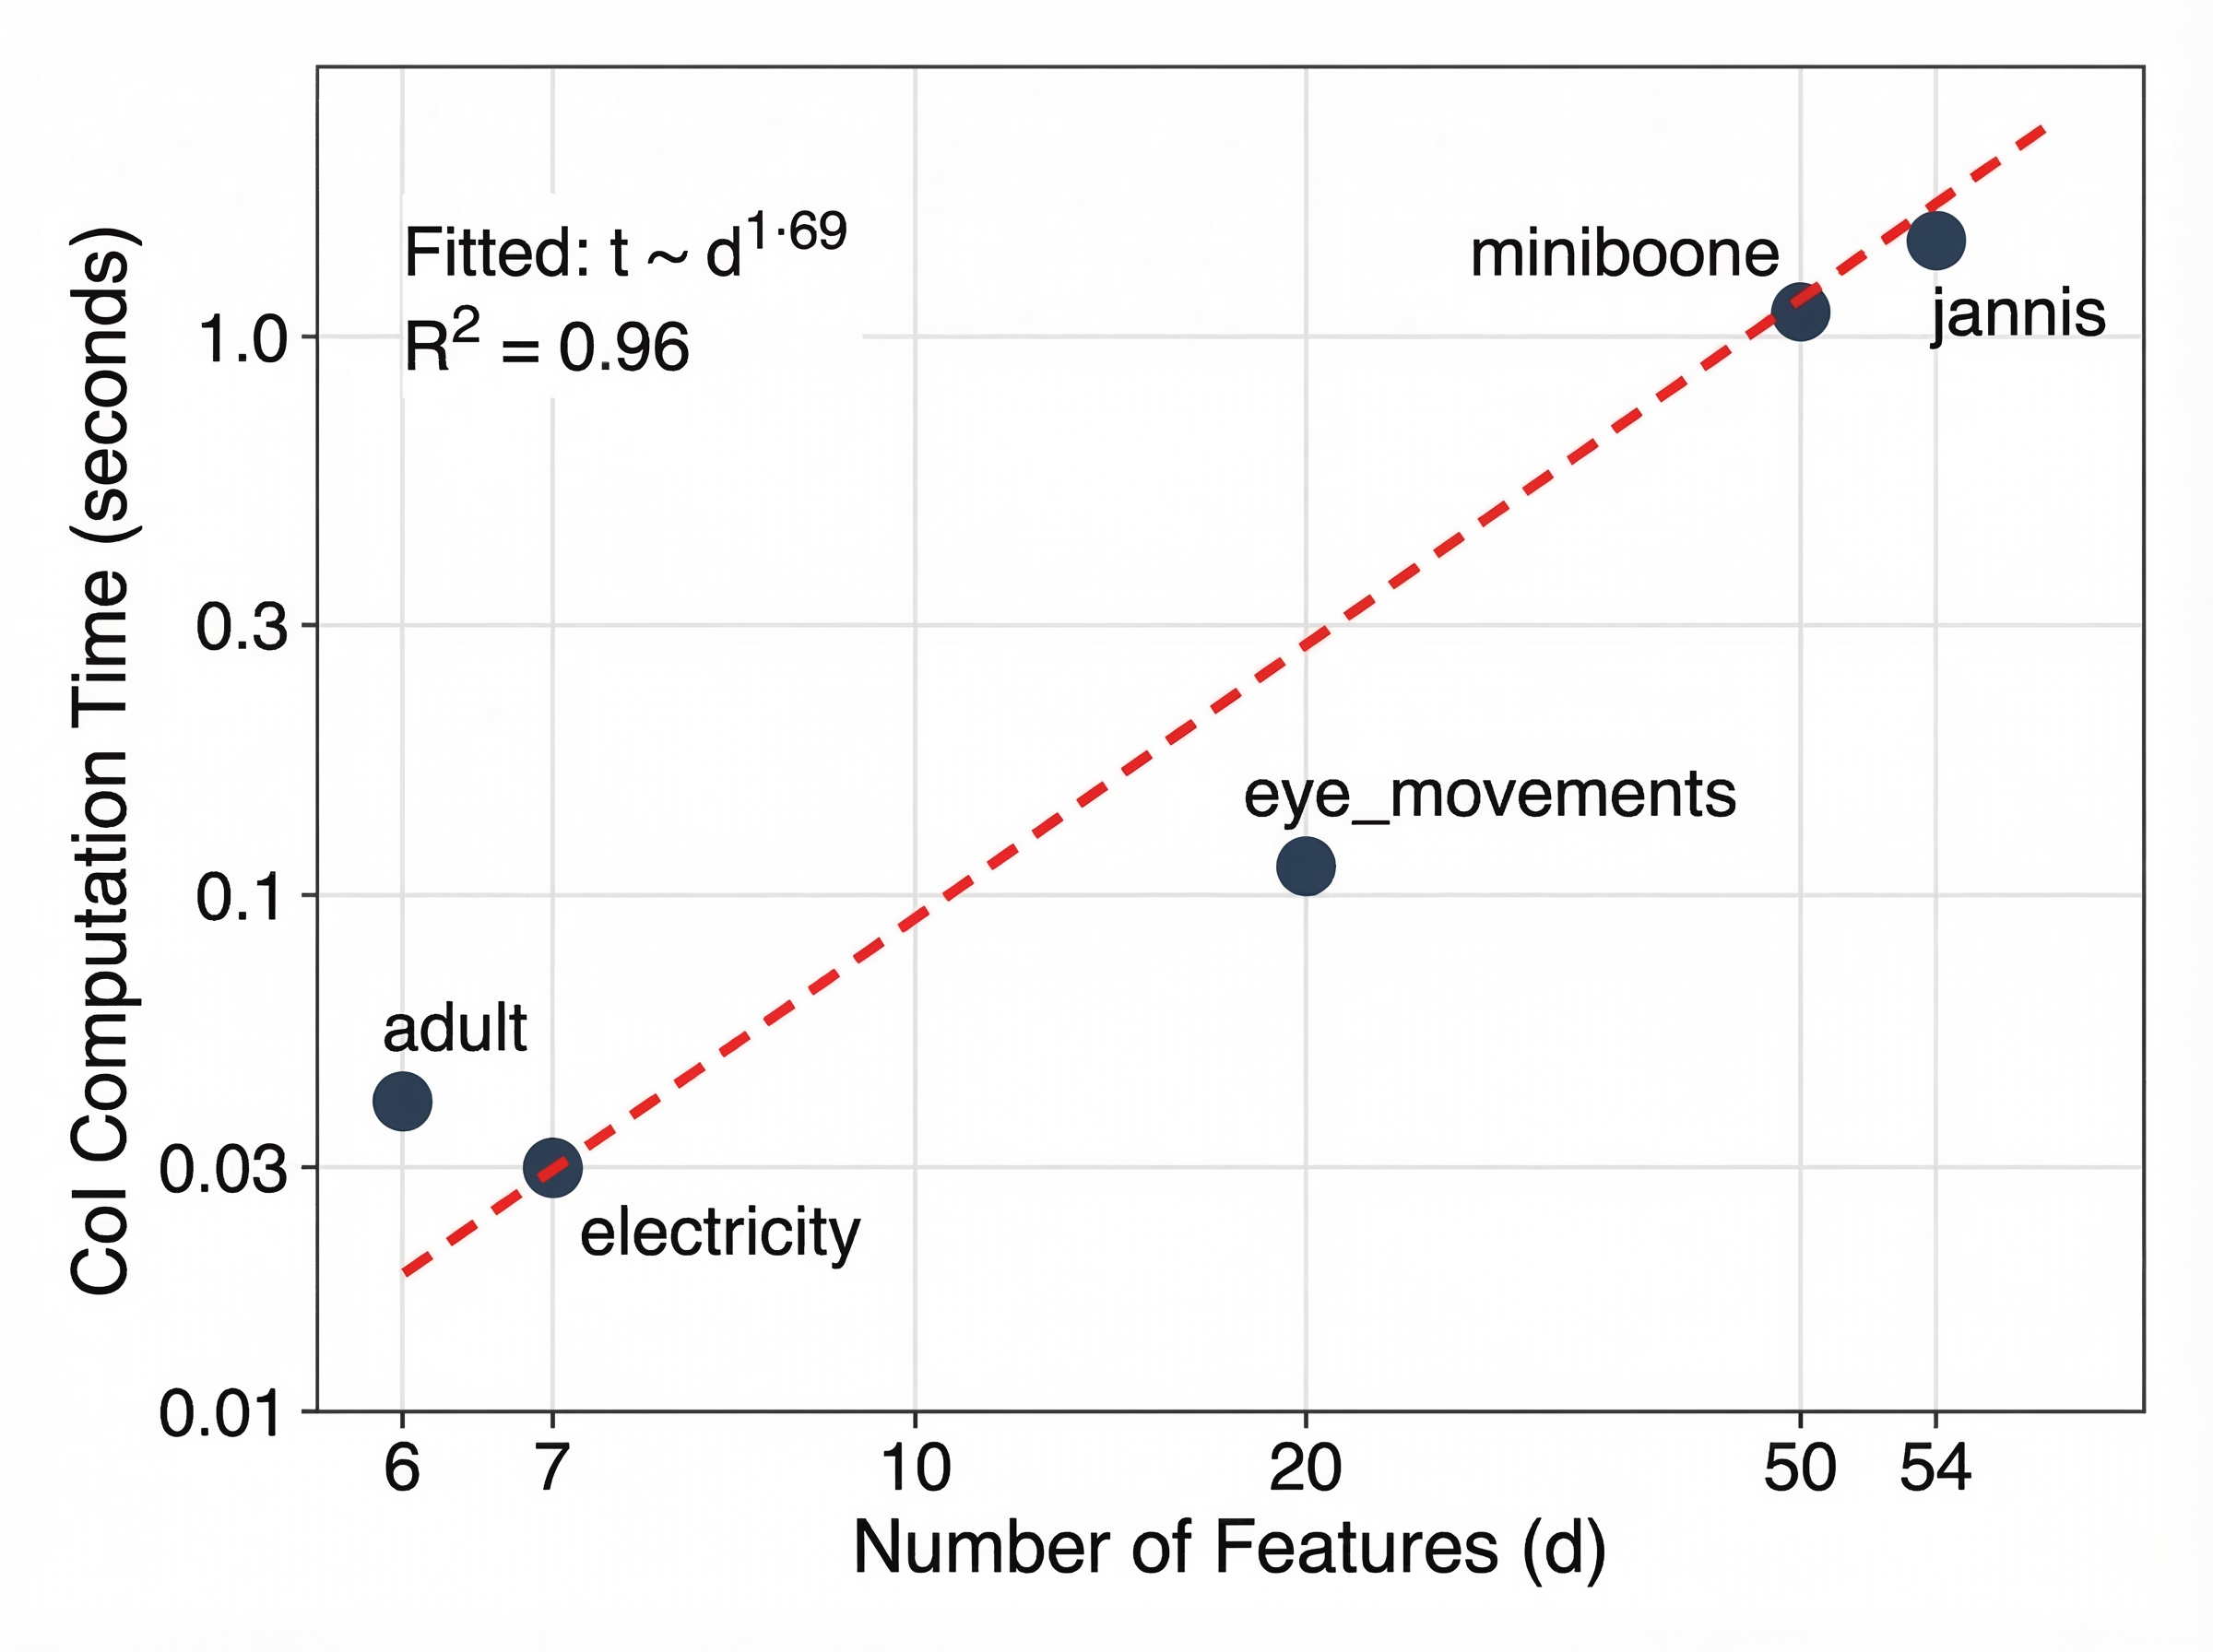
\includegraphics[width=0.92\textwidth,max height=0.4\textheight]{figures/fig_5_v0.png}
  \caption{Log-log plot of Co-Information computation time versus number of features $d$ across 5 benchmark datasets. The fitted power law $t \propto d^{1.69}$ ($R^2 = 0.96$) is consistent with the theoretical $O(d^2 \cdot n)$ complexity. The maximum single-dataset pipeline time is 8.1 minutes (miniboone, $d{=}50$, $n{=}72{,}998$).}
  \label{fig:scaling}
\end{figure}

Co-Information computation time scales as $O(d^{1.69})$ in features ($R^2 = 0.96$), consistent with the theoretical $O(d^2 \cdot n)$ complexity given that sample sizes vary across datasets. The maximum single-dataset pipeline time is 8.1 minutes (miniboone, $d{=}50$, $n{=}72{,}998$), well within practical bounds. Per-dataset CoI computation times range from 0.03 seconds (electricity, $d{=}7$) to 1.24 seconds (jannis, $d{=}54$). Spectral clustering adds negligible overhead ($< 0.5$ seconds for all datasets). FIGS tree fitting dominates the total runtime, ranging from 0.1 to 3.95 seconds per fold. All FIGS variants are faster than EBM on all 8 datasets, with a geometric mean speedup of 21.25$\times$.

%---------------------------------------------------------------------
\section{Discussion}
\label{sec:discussion}
%---------------------------------------------------------------------

\paragraph{What works.} The core idea of using spectral decomposition of Co-Information feature interaction graphs to constrain oblique tree splits is validated as both novel and functional. Co-Information correctly identifies synergistic features that have zero marginal MI, solving the fundamental pre-filtering contradiction of the prior SG-FIGS approach. Spectral clustering discovers meaningful feature modules: on synthetic data with planted XOR structure, the pipeline achieves perfect module recovery (Jaccard $= 1.0$) on easy and medium variants. On real benchmarks, spectral-guided oblique FIGS ranks highest among all FIGS variants (average rank 4.43 versus 5.29 for random oblique and 6.14 for axis-aligned), with the advantage most pronounced on higher-dimensional datasets such as miniboone ($d{=}50$, accuracy 0.902 vs.\ 0.887 for random oblique) and jannis ($d{=}54$, accuracy 0.741 vs.\ 0.734). The information-theoretic grounding ensures that features are combined based on their interaction structure rather than arbitrarily.

\paragraph{What fails and why.} The signed spectral clustering mechanism---the theoretical centerpiece connecting social balance theory to feature interaction analysis---does not improve over unsigned spectral clustering. The root cause is a fundamental incompatibility between Co-Information sign estimation and the SPONGE algorithm. Three independent bias mechanisms produce predominantly negative CoI values regardless of the true interaction type, causing the positive Laplacian $L^+$ to degenerate. This failure mode is informative: it reveals that the sign structure of information-theoretic interaction matrices is unreliable with current estimation methods, and that unsigned spectral clustering, which uses only edge magnitudes, is the appropriate algorithm for this application.

\paragraph{Limitations.} Several limitations warrant discussion. (1)~All main experiments used quantile binning for MI estimation; KSG estimators produce different CoI sign distributions and may rescue signed spectral methods, but this alternative was not evaluated end-to-end. (2)~Real datasets span $d{=}6$ to $d{=}54$; the pipeline has not been validated on datasets with hundreds of features, though synthetic tests at $d{=}200$ show feasibility. (3)~The pairwise Co-Information assumption ignores higher-order interactions (3-way, 4-way synergies), which may be important for some datasets. (4)~The eigengap-based $k$-selection method systematically underestimates the number of modules on high-dimensional data. (5)~The comparison includes EBM and Random Forest as baselines but not other interaction-aware methods such as PIDF \citep{Westphal2025} or Interaction Forests \citep{Hornung2022}.

\paragraph{Broader implications.} The negative result regarding signed spectral clustering on information-theoretic graphs has implications beyond oblique trees. Any method that constructs a signed graph from MI-based pairwise interactions and applies signed graph clustering (balance theory, SPONGE, or matrix power means \citep{Mercado2019}) must account for estimator-induced sign bias. Our work provides both a diagnosis of this problem and a practical solution: use unsigned spectral clustering on the absolute Co-Information matrix.

%---------------------------------------------------------------------
\section{Conclusion}
\label{sec:conclusion}
%---------------------------------------------------------------------

We introduced a pipeline that uses spectral decomposition of pairwise Co-Information graphs to provide principled feature grouping for oblique decision tree splits. Evaluated across 6 synthetic and 8 real-world datasets with 28 statistical tests, the approach achieves accuracy equivalent to random oblique baselines (Bayesian $P(\text{ROPE}) = 0.996$) while using information-theoretically grounded feature modules. Unsigned spectral clustering on absolute Co-Information values is the recommended algorithm, as signed spectral methods (SPONGE) fail due to systematic MI estimator bias.

The work opens several directions for future research:
\begin{itemize}
  \item Evaluating the pipeline with KSG estimators end-to-end to test whether corrected sign distributions rescue signed spectral clustering.
  \item Extending to higher-order Co-Information (3-way, 4-way) to capture interactions beyond pairwise structure.
  \item Developing adaptive $k$-selection methods for spectral clustering on information-theoretic graphs.
  \item Scaling evaluation to datasets with hundreds of features to test the practical limits of the $O(d^2 \cdot n)$ pipeline.
\end{itemize}

\bibliographystyle{plainnat}
\bibliography{references}

\end{document}
